\documentclass[11pt,a4paper]{article}

\usepackage[margin=1in]{geometry}
\usepackage{amsmath}
\usepackage{amssymb}
\usepackage{graphicx}
\usepackage[T1]{fontenc}
\usepackage[utf8]{inputenc}
\usepackage{lmodern}
\usepackage[hidelinks]{hyperref}

\graphicspath{{docs/images/algorithms/}{../images/algorithms/}}

\title{Cycle Analysis in EvalData\\A Small Algorithm Note}
\author{EvalData Repository Example}
\date{April 2026}

\begin{document}

\maketitle

\section{Purpose}

This note explains the current cycle-analysis workflow in EvalData. The examples use the built-in spectral demo, which includes a deterministic impact marker and repeated ringing events.

Cycle analysis in EvalData is based on segmentation first and statistics second. The quality of the result depends strongly on whether the cycle boundaries are meaningful.

\section{Two Cycle Modes}

The current UI exposes four modes:

\begin{itemize}
    \item \textbf{fixed\_length}: build cycles as equal row blocks,
    \item \textbf{rising\_edge}: detect cycle starts from threshold crossings on a reference signal,
    \item \textbf{zero\_crossing}: detect cycles between sign-change points of a reference signal,
    \item \textbf{peak}: detect cycles between successive peaks of a reference signal.
\end{itemize}

\subsection{Fixed-Length Segmentation}

For a chosen cycle length $L$, the data is split into half-open intervals

\[
[0,L), [L,2L), [2L,3L), \dots
\]

until there are not enough rows left to form another full cycle.

\subsection{Rising-Edge Segmentation}

For reference signal $r[n]$ and threshold $\tau$, EvalData first marks samples above threshold:

\[
b[n] = \mathbf{1}_{\{r[n] \ge \tau\}}.
\]

A rising edge occurs when

\[
b[n] = 1 \quad \text{and} \quad b[n-1] = 0.
\]

Consecutive rising edges define candidate cycle ranges. Short ranges below the configured minimum length are discarded.

\begin{figure}[ht]
    \centering
    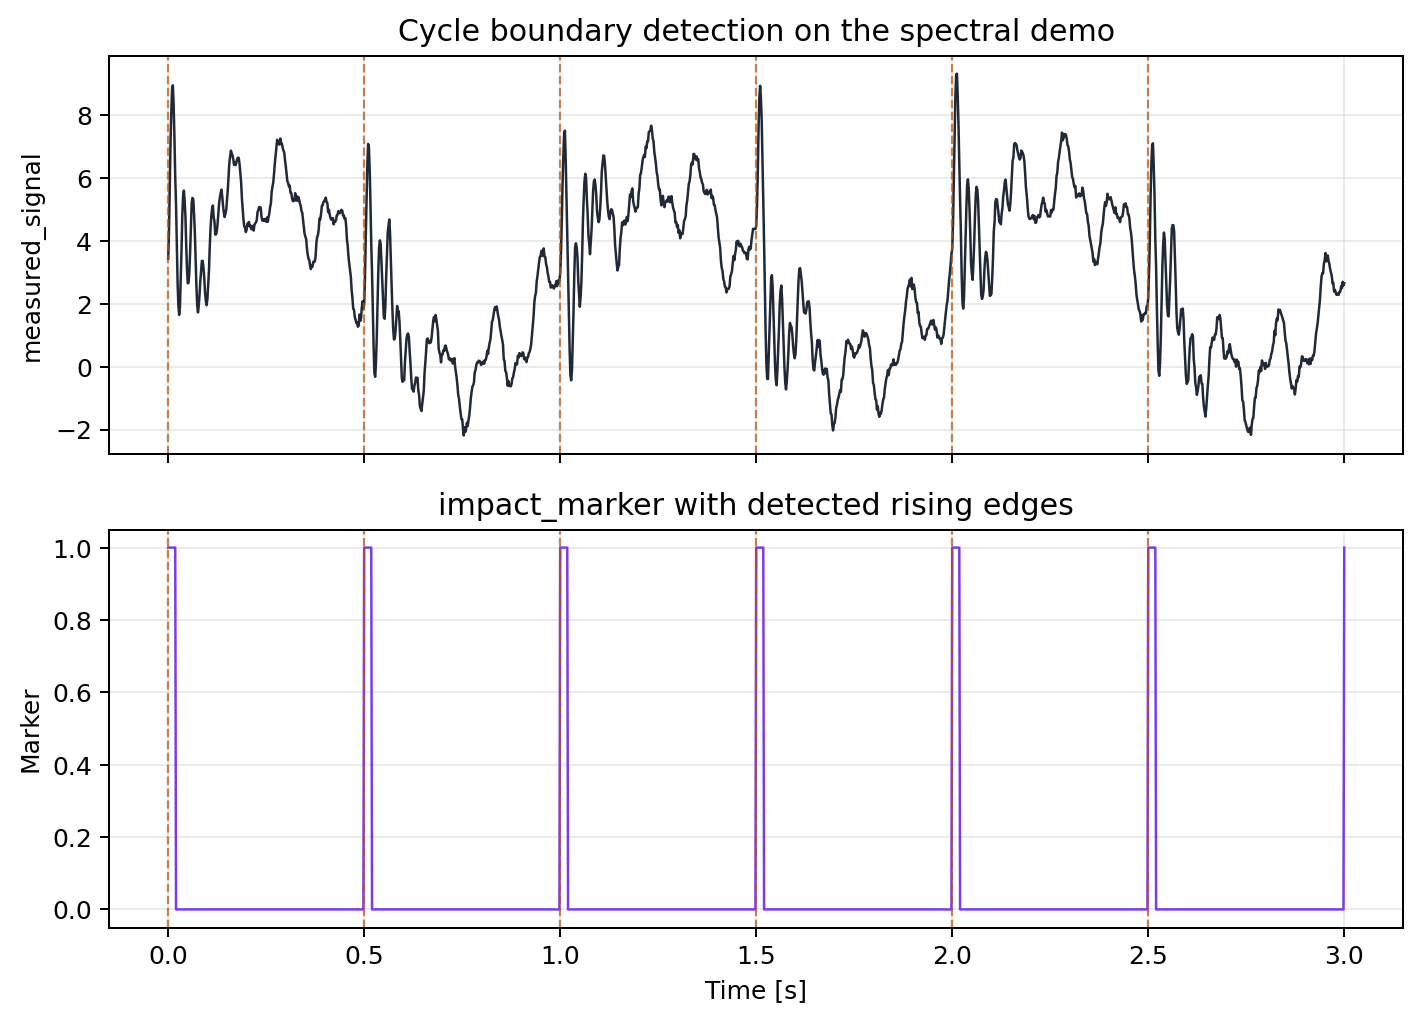
\includegraphics[width=0.92\linewidth]{cycle_detection_example.png}
    \caption{Rising-edge cycle detection on the built-in spectral demo. The marker channel provides explicit threshold crossings for cycle boundary detection.}
\end{figure}

\subsection{Zero-Crossing Segmentation}

For a reference signal $r[n]$, a zero crossing occurs where the sign of $r$ changes between consecutive samples. EvalData computes the sign-change indicator

\[
\Delta s[n] = \mathrm{sign}(r[n]) - \mathrm{sign}(r[n-1]).
\]

Crossings are classified by the user-selected direction:

\begin{itemize}
    \item \textbf{rising}: $\Delta s[n] > 0$ (signal crosses from negative to positive),
    \item \textbf{falling}: $\Delta s[n] < 0$ (signal crosses from positive to negative),
    \item \textbf{both}: $\Delta s[n] \ne 0$ (any sign change).
\end{itemize}

Consecutive crossing indices define candidate cycle ranges. A minimum cycle length parameter allows short spurious segments to be discarded.

\subsubsection{Parameters}

\begin{itemize}
    \item \textbf{Reference column}: the signal on which zero crossings are detected.
    \item \textbf{Direction}: \texttt{rising}, \texttt{falling}, or \texttt{both}.
    \item \textbf{Minimum cycle length}: ranges shorter than this many samples are dropped.
    \item \textbf{Maximum cycles} (optional): cap the number of detected cycles.
\end{itemize}

\subsection{Peak-Based Segmentation}

Peak-based cycle detection finds successive local maxima of a reference signal using \texttt{scipy.signal.find\_peaks} and defines each cycle as the interval between consecutive peaks.

A peak at sample $n$ satisfies

\[
r[n] > r[n-1] \quad \text{and} \quad r[n] > r[n+1],
\]

subject to optional constraints. Consecutive peak indices $p_i, p_{i+1}$ yield cycle ranges $[p_i, p_{i+1})$.

\subsubsection{Prominence Filtering}

Prominence measures how much a peak stands out from surrounding valleys. For a peak at index $p$, the prominence is

\[
\mathrm{prom}(p) = r[p] - \max\bigl(\text{highest valley on left}, \text{highest valley on right}\bigr).
\]

Setting a minimum prominence value filters out small local maxima caused by noise, retaining only structurally significant peaks as cycle boundaries.

\subsubsection{Parameters}

\begin{itemize}
    \item \textbf{Reference column}: the signal on which peaks are detected.
    \item \textbf{Minimum cycle length}: enforced as a minimum distance between peaks.
    \item \textbf{Prominence} (optional): minimum peak prominence; peaks below this threshold are ignored.
    \item \textbf{Maximum cycles} (optional): cap the number of detected cycles.
\end{itemize}

\section{Cycle Alignment}

Once valid cycle ranges are collected, EvalData converts each range into a numeric array. Because detected cycles may differ slightly in length, the current implementation aligns them by truncating every cycle to the shortest valid cycle length:

\[
L_{\text{align}} = \min_i L_i.
\]

This yields a cycle matrix

\[
X \in \mathbb{R}^{M \times L_{\text{align}}},
\]

where $M$ is the number of detected cycles.

\section{Per-Cycle Metrics}

For each cycle $x_i[n]$, EvalData reports:

\[
\mu_i = \frac{1}{L_i} \sum_{n=0}^{L_i-1} x_i[n],
\]

\[
\sigma_i = \sqrt{\frac{1}{L_i-1} \sum_{n=0}^{L_i-1} (x_i[n] - \mu_i)^2},
\]

\[
\mathrm{RMS}_i = \sqrt{\frac{1}{L_i} \sum_{n=0}^{L_i-1} x_i[n]^2},
\]

\[
\mathrm{P2P}_i = \max_n x_i[n] - \min_n x_i[n].
\]

Minimum and maximum values are also stored per cycle.

\section{Representative Cycle}

After alignment, EvalData computes a representative cycle summary across the cycle matrix column by column:

\[
\bar{x}[k] = \frac{1}{M} \sum_{i=1}^{M} X_{ik},
\]

with corresponding standard deviation, minimum, and maximum at each aligned step $k$.

\begin{figure}[ht]
    \centering
    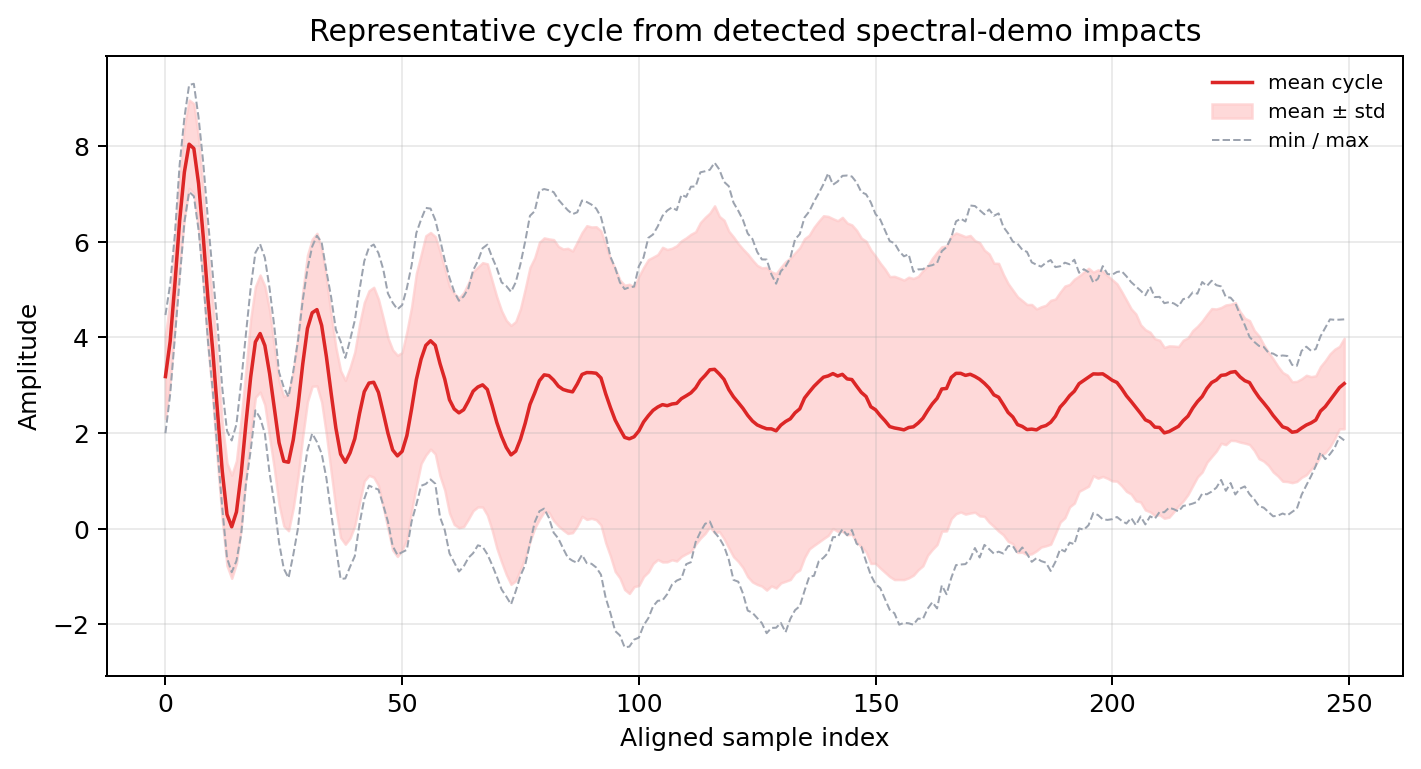
\includegraphics[width=0.92\linewidth]{cycle_representative_example.png}
    \caption{Representative cycle summary from detected spectral-demo impacts. The band shows mean $\pm$ standard deviation across aligned cycles.}
\end{figure}

\section{What the Demo Shows}

The spectral demo repeats impacts every 0.5 seconds and adds decaying ringing after each event. That makes it a good control case for both segmentation strategies:

\begin{itemize}
    \item a fixed length of 250 rows matches 0.5 seconds at 500 Hz,
    \item the impact marker allows explicit threshold-based cycle detection.
\end{itemize}

\section{Practical Interpretation Limits}

\begin{itemize}
    \item Fixed-length segmentation is only valid if the cycle length is known or approximately constant.
    \item Rising-edge detection depends on threshold choice and signal cleanliness.
    \item Zero-crossing detection requires the reference signal to actually oscillate around zero; a nonzero offset must be removed first.
    \item The \texttt{both} direction for zero crossings produces half-cycles rather than full oscillation periods.
    \item Peak-based detection is sensitive to noise; without adequate prominence filtering, spurious peaks create meaningless short cycles.
    \item Truncating all cycles to the shortest length simplifies alignment but discards tail samples from longer cycles.
    \item Cycle metrics summarize segments; they do not prove physical repeatability by themselves.
\end{itemize}

\section{Conclusion}

EvalData's cycle workflow is deliberately simple: detect or define cycle ranges, align them, and summarize them. Four detection strategies are available---fixed length, rising edge, zero crossing, and peak-based---so the user can match the segmentation logic to the physical structure of the signal. The mathematical assumptions behind the chosen segmentation step should always be stated explicitly.

\begin{thebibliography}{9}

\bibitem{bendat2010}
J.~S.~Bendat and A.~G.~Piersol,
\emph{Random Data: Analysis and Measurement Procedures}, 4th~ed.
Hoboken, NJ: Wiley, 2010.

\bibitem{downing1982}
S.~D.~Downing and D.~F.~Socie,
``Simple rainflow counting algorithms,''
\emph{International Journal of Fatigue}, vol.~4, no.~1, pp.~31--40, 1982.

\bibitem{scipy_find_peaks}
SciPy Community,
``scipy.signal.find\_peaks,'' SciPy Reference Guide.
Available: \url{https://docs.scipy.org/doc/scipy/reference/generated/scipy.signal.find_peaks.html}

\end{thebibliography}

\end{document}